%ctrl+alt+m:open Math Preview
\documentclass[a4paper,11pt,uplatex]{jsarticle}%titlepage
%:/usr/local/texlive/texmf-local/tex/latex/report/report.sty
\usepackage{myreport}
\title{拡散モデル(Diffusion Model)を理解するために}
\author{20B01392 松本侑真}
\date{\today}
\begin{document}
\maketitle
\begin{abstract}
近年、機械学習を応用した生成系AIがブームである。
生成系AIを使うことで、プロンプトに入力したテキストデータから画像データなどを出力することができる。
拡散モデルを用いた有名な生成系AIのStable Diffusionでは、無料でプロンプトに入力した文字(例:かわいい犬)から、かわいい犬の画像を出力することができる。
このような生成系AIで用いられる拡散モデルについて理解するための基礎を説明する。
\end{abstract}
\tableofcontents
\newpage

\section{生成モデルでは何を行っているのか}
生成モデル(拡散モデル)は、事前に与えられた教師データを元にモデルを学習することで、
未知の入力に対して最適化された出力をアウトプットすることができる。
例えば、いろいろな人間の顔データを学習させた生成モデルを用いると、
「40歳のおじさん」や「20代のアイドル」といった入力を元にして、学習されたモデルで生成した顔画像を出力する。

生成モデルの学習というのは、「モデルの入力から欲しいデータを生み出す確率分布」をいかにして見つけるかということである。
すなわち、任意のデータ$\vv{x}$は、とある1つの確率分布$p(\vv{x})$に従って生み出されるという仮定のもと、自分のモデルをその$p(\vv{x})$に限りなく近づけることが生成モデルにおける学習である。
すなわち、あらゆるデータが従う確率分布$p(\vv{x})$そのものを手に入れることができれば、$p(\vv{x})$の値を出力するような$\vv{x}$を見つけることが可能であるだろう。
これによって、$p(\vv{x})=\text{「20代のアイドル」}$を満たす画像$\vv{x}$を出力することができる。

\subsubsection*{学習を行う前に得られているもの}
モデルの学習を行うためには、そのための学習データが必要である。$n$個の学習データ$\vv{x}_1,\,\vv{x}_2,\,\cdots,\,\vv{x}_n$が手元にあるとする。
このとき、
\begin{equation}
  p_0(\vv{x}) = \frac{1}{n}\sum_{i=1}^{n}\delta(\vv{x}-\vv{x}_i)
\end{equation}
を経験分布と呼ぶ。この経験分布は、$n$が十分に大きいとき、あらゆるデータを生み出す確率分布$p(x)$に非常に近いであろう:
\begin{equation}
  p_0(\vv{x}) \approx p(\vv{x})\;。
\end{equation}
なお、データを連続変数として扱う場合は$\delta(\vv{x}-\vv{x}_i)$をデルタ関数、離散変数として扱う場合はクロネッカーのデルタとして扱う。

\subsubsection*{学習のために必要なもの}
生成モデルにおいて学習させるための確率分布は自ら用意する必要がある。すなわち、パラメータ$\theta$を用いて、
\begin{equation}
  p(\vv{x})\approx q_{\theta}(\vv{x})
\end{equation}
となるようなモデル$q_{\theta}(\vv{x})$を見つけたい。モデル$q_{\theta}(\vv{x})$の関数形は計算しやすい形を用いて、
パラメータ$\theta$を最適化することで$p(\vv{x})$に近づけるというアプローチを取る。

\section{ボルツマンマシン}
ボルツマンマシンとは、モデル$q_{\theta}(\vv{x})$が
\begin{equation}
  q_{\theta}(\vv{x}) = \frac{1}{Z_{\theta}}\exp(-E_{\theta}(\vv{x}))\;。
\end{equation}
と表されるものである。このような関数形をGibbs-Boltzmann分布(指数関数分布族)と呼ぶ。
ここで、規格化定数$Z_{\theta}$は
\begin{equation}
  Z_{\theta} = \sum_{\vv{x}}\exp(-E_{\theta}(\vv{x}))
\end{equation}
である。このように定義された$q_{\theta}(\vv{x})$を$p(\vv{x})$に近づけることが目標である。
しかし、$p(\vv{x})$の形は誰も知らない。今手元にあるのは経験分布$p_0(\vv{x})$だけである。
そのため、学習データの数$n$が十分に多いとして、$q_{\theta}(\vv{x})$を経験分布$p_0(\vv{x})$に近づけることを行う。

\subsection{Kullback-Leibler情報量}
学習を行うためには、2つの確率分布$p(\vv{x}),\,q(\vv{x})$の近さを定義する必要がある。
この「近さ」は、データ$\vv{x}$を入力した際の2つの確率分布間の「距離$D(p\parallel q)$」を測ることで定義することができるだろう。
このような関数$D(p\parallel q)$はどのように設定しても良いのだが、
今回は、Kullback-Leibler divergence(KL情報量)$D_{\text{KL}}(p\parallel q)$を導入する:
\begin{equation}
  D_{\text{KL}}(p(\vv{x})\parallel q(\vv{x})) = \sum_{\vv{x}}p(\vv{x})\ln\frac{p(\vv{x})}{q(\vv{x})}\;。
\end{equation}
KL情報量には
\begin{enumerate}
  \renewcommand{\labelenumi}{(\roman{enumi}).}
  \item $D(p\parallel q)\geq 0$(等号成立は$p=q$のとき)
  \item $D(p\parallel q) \neq D(q\parallel p)$(非対称性)
\end{enumerate}
といった性質がある。特に、KL情報量は$0$以上であるといった性質を良く用いる。この性質を2つの方法で証明してみる。
\subsubsection*{Gibbsの不等式を用いる方法}
Gibbsの不等式とは、$x>0$において
\begin{equation}
  x-1\geq \ln{x}\Longleftrightarrow \ln{\frac{1}{x}}\geq 1-x
\end{equation}
が成立する不等式である。
\begin{figure}[H]
  \centering
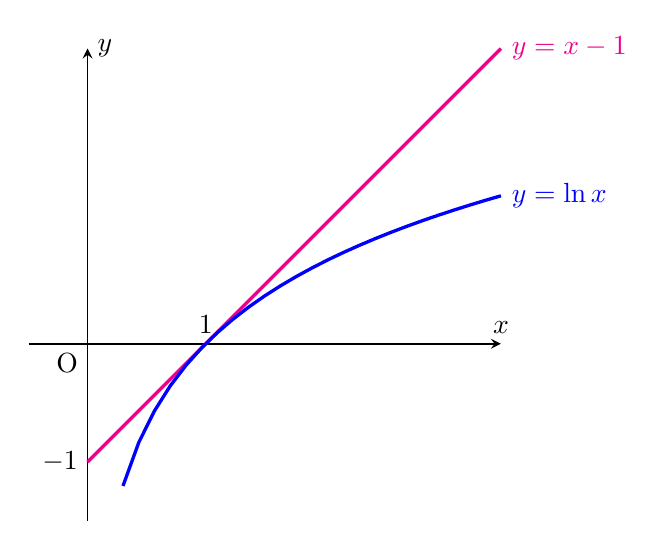
\begin{tikzpicture}[scale=1.5]
  \draw[->,>=stealth,semithick](-0.5,0)--(3.5,0)node[above]{$x$};%x軸
  \draw[->,>=stealth,semithick](0,-1.5)--(0,2.5)node[right]{$y$};%y軸
  \draw(0,0)node[below left]{O};%原点
  \draw(1,0)node[above]{$1$};
  \draw(0,-1)node[left]{$-1$};
  \draw[magenta,very thick,domain=0:3.5]plot(\x,\x-1)node[right]{$y=x-1$};
  \draw[blue,very thick,domain=0.3:3.5]plot(\x,{ln(\x)})node[right]{$y=\ln{x}$};
  \end{tikzpicture}
  \caption{Gibbsの不等式の直感的な理解}
\end{figure}
Gibbsの不等式を用いると、
\begin{equation}
  D_{\text{KL}}(p\parallel q) = \sum_{\vv{x}}p(\vv{x})\ln\frac{p(\vv{x})}{q(\vv{x})}
  \geq \sum_{\vv{x}}p(\vv{x})\qty(1-\frac{q(\vv{x})}{p(\vv{x})}) 
  = \sum_{\vv{x}}p(\vv{x})-\sum_{\vv{x}}q(\vv{x}) =0
\end{equation}
と示される。
\newpage
\subsubsection*{Jensenの不等式を用いる方法}
Jensenの不等式とは、上に凸な関数$f(x)$に対して、
\begin{equation}
  f\qty(\frac{a+b}{2})\geq \frac{f(a)+f(b)}{2}
\end{equation}
が成立する不等式である。
\begin{figure}[H]
  \centering
\begin{tikzpicture}[scale=1.5]
  \coordinate(A)at(-2,0);
  \coordinate(B)at(1,0);
  \draw[->,>=stealth,semithick](-3.5,0)--(3.5,0)node[above]{$x$};%x軸
  \draw[magenta,very thick,domain=-3:3]plot(\x,{-0.3*(\x-3)*(\x+3)});
  \coordinate(YA)at(-2,1.5);
  \coordinate(YB)at(1,2.4);
  \draw[dashed](A)node[below]{$a$}--(YA);
  \draw[dashed](B)node[below]{$b$}--(YB);
  \draw[dashed](YA)--(YB);
  \fill(YA)circle(0.05);
  \fill(YB)circle(0.05);
  \coordinate(XAB)at($(A)!1/2!(B)$);
  \coordinate(YAB)at($(XAB)+(0,0.3*7/2*5/2)$);
  \draw[dashed](XAB)node[below]{$\frac{a+b}{2}$}--(YAB);
  \fill(YAB)circle(0.05);
  \end{tikzpicture}
  \caption{Jensenの不等式の直感的な理解}
\end{figure}
Jensenの不等式を用いると、
\begin{equation}
  D_{\text{KL}}(p\parallel q) = -\sum_{\vv{x}}p(\vv{x})\ln\frac{q(\vv{x})}{p(\vv{x})}
  \geq -\ln\qty(\sum_{\vv{x}}p(\vv{x})\frac{q(\vv{x})}{p(\vv{x})}) = 0
\end{equation}
と示される。

\subsection{例:ガウス分布のKL情報量と学習}
モデル$q_{\theta}(\vv{x})$をガウス分布とおいて最適化を行う。人間が計算できるのはせいぜいガウス分布程度であるため、
これ以上難しいモデルは考えない。まずは$\vv{x}$が1次元のスカラーである場合を考える:
\begin{equation}
  q_{\theta}(x)\propto \exp\qty(-\frac{1}{2\sigma^2}(x-\mu)^2)\;。
\end{equation}
規格化定数は
\begin{equation}
  Z_{\theta}=\int_{-\infty}^{\infty}dx\,\exp\qty(-\frac{1}{2\sigma^2}(x-\mu)^2) = \sqrt{2\pi\sigma^2}
\end{equation}
となる。したがって、
\begin{equation}
  q_{\theta}(x)=\frac{1}{\sqrt{2\pi\sigma^2}}\exp\qty(-\frac{1}{2\sigma^2}(x-\mu)^2)
\end{equation}
となる。このモデルの未知数は$\mu$と$\sigma^2$であるため、最適化すべきパラメータは$\theta=\{\mu,\,\sigma^2\}$となる。
次に、KL情報量を考える。$q_{\theta}(x)$を$p(x)$に近づけることができれば良いのだが、あいにく$p(x)$の具体形はわからない。
そのため、経験分布$p_0(x)=\sum_{i=1}^n\delta(x-x_i)$にモデルを近づけることを考える。KL情報量を計算すると、
\begin{align}
  D_{\text{KL}}(p_0\parallel q_{\theta}) = \int dx\,p_0(x)\qty(\ln{p_0(x)}-\ln{q_{\theta}(x)})
  &\underbrace{=}_{\theta\text{のみ}} -\int dx\,p_0(x)\qty(\frac{1}{2\sigma^2}(x-\mu)^2+\frac{1}{2}\ln{\sigma^2}) \notag \\
  &\;\,=\frac{1}{2\sigma^2}\frac{1}{n}\sum_{i=1}^n(x_i-\mu)^2+\frac{1}{2}\ln{\sigma^2}
\end{align}
となる。KL情報量を最小化(学習)すれば、経験分布に近いモデルが得られるため、$\mu$と$\sigma^2$で偏微分を行う。
\begin{align}
  \pdv{D_{\text{KL}}}{\mu} &= -\frac{1}{\sigma^2}\frac{1}{n}\sum_{i=1}^{n}(x_i-\mu) = 0
  &&\Longleftrightarrow \mu = \frac{1}{n}\sum_{i=1}^nx_i\;\text{(データの平均)} \\
  \pdv{D_{\text{KL}}}{\sigma^2} &= -\frac{1}{2(\sigma^2)^2}\frac{1}{n}\sum_{i=1}^n(x_i-\mu)^2 + \frac{1}{2\sigma^2}=0
  &&\Longleftrightarrow \sigma^2 = \frac{1}{n}\sum_{i=1}^n(x_i-\mu)^2\;\text{(データの分散)}
\end{align}
この結果からわかることは、ガウス分布のモデルの平均$\mu$はデータの平均値に、モデルの分散$\sigma^2$はデータの分散にすれば、
$p(x)$に近いモデル$q_{\theta}(x)$を生成できるということである。

\subsection{最尤法(=KL最小化)}
最尤法とは、KL情報量の最小化と同値なものであるが、良く使われるため紹介する。モデルの学習は、
\begin{equation}
  \min_{\theta}\qty{D_{\text{KL}}(p_0(\vv{x})\parallel q_{\theta}(\vv{x}))} 
  = \max_{\theta}\qty{\sum_{\vv{x}}p(\vv{x})\ln{q_{\theta}(\vv{x})}} 
  = \max_{\theta}\qty{\frac{1}{n}\sum_{i=1}^n\ln{q_{\theta}(\vv{x}_i)}}
\end{equation}
と変形することができる。$\ln{q_{\theta}(\vv{x}_i)}$を対数尤度関数と呼び、モデルの良さの指標として使われる。
対数尤度を最大化することは、KL情報量の最小化と同値なものである。
\subsection{高次元化}

\section{隠れ変数を導入してリッチなモデルへ}

\section{制限ボルツマンマシン}

\section{マルコフ連鎖モンテカルロ法(MCMC)}

\section{交換モンテカルロ法}

\section{MCMCを用いないボルツマンマシン}

\section{変分オートエンコーダー}

\section{階層変分オートエンコーダ}

\end{document}